\documentclass[11pt]{report}
\usepackage[english]{babel}
\usepackage[utf8x]{inputenc}
\usepackage{multicol}
\usepackage[nottoc]{tocbibind}
\usepackage{caption}

\newcommand{\me}{\mathrm{e}}
\usepackage{amsmath}
\usepackage{tabularx}
\usepackage{setspace}
\usepackage{natbib}
\usepackage{multicol}
\usepackage{ragged2e}
\usepackage{graphicx}
%\usepackage[toc,page]{appendix}
\usepackage[colorinlistoftodos]{todonotes}
\oddsidemargin 1.2cm
\evensidemargin 0.5cm

\begin{document}

\begin{titlepage}

\newcommand{\HRule}{\rule{\linewidth}{0.5mm}}

\center % Center everything on the page
 
% Name of your university/college
\textsc{\Large \textbf{An Improved Grey Wolf Optimizer \\[0.25cm]Based on Tracking and
Seeking Modes\\[0.25cm] to Solve Function Optimization \\[0.25cm]Problems}}\\[0.75cm] % Major heading 

{ \it A seminar report submitted to Rajagiri School of Engineering \& Technology\\ in partial fulfilment of degree of \\[0.75cm]B.Tech.\\[0.5cm]}{in\\[0.5cm] Electronics \& Communication Engineering\\[0.75cm]by}\\[0.5cm]\textsc{\textbf{Varsha Ramdas \\[0.35cm]Roll No: RET17EC177}}\\[1cm] % Minor heading such as course title



\includegraphics[width=2.5cm]{Rset Vertical.jpg}\\[1cm]
 
\textsc{DEPARTMENT OF ELECTRONICS \& COMMUNICATION ENGINEERING\\[0.15cm]\textsc{\textbf{RAJAGIRI SCHOOL OF ENGINEERING \& TECHNOLOGY}}\\[0.15cm]kerala\\[0.15cm]}{JANUARY 2021}

\end{titlepage}

\vfill % Fill the rest of the page with whitespace
\thispagestyle{empty}

\vspace*{-0.3cm}
\begin{center}
{\large \bf  DEPARTMENT OF ELECTRONICS \& COMMUNICATION ENGINEERING}\vspace{0.1cm}
\end{center}

\begin{center} 
{\Large \bf RAJAGIRI SCHOOL OF ENGINEERING \& TECHNOLOGY}\vspace{0.1cm}
\end{center}

\begin{center} 
{\large \bf KOCHI - 682039, }\vspace{0.1cm}
\end{center}

\begin{figure}[hbt]
\centering
\centerline{
\includegraphics[scale=0.6]{Rset Vertical.jpg}}
\end{figure}

\begin{center} 
{\Large \textit {Certificate}}\vspace{.1cm}
\end{center}

\justify
\doublespace
\textit {This is to certify that this report entitled ``An Improved Grey Wolf Optimizer Based on Tracking and
Seeking Modes to Solve Function Optimization Problems'' is a bonafide record of the seminar presented by \textbf{Ms. Varsha Ramdas, Roll No. RET17EC177} under our guidance towards the partial fulfilment of the requirements for the award of \textbf{Bachelor of Technology in Electronics \& Communication Engineering} of the \textbf{APJ Abdul Kalam Technological University}.}
\vspace{0.4cm}

\begin{minipage}{0.45\textwidth}
\begin{flushleft} \large
\textbf{Mr. Abhishek Viswakumar}\\
Assistant Professor\\
Dept. of ECE\\
RSET\\
Kochi
\end{flushleft}
\end{minipage}
~
\begin{minipage}{0.4\textwidth}
\begin{flushright} \large
\textbf{Dr. Rithu James}\\
Head of Department\\
Dept. of ECE\\
RSET\\
Kochi
\end{flushright}
\end{minipage}
%~
\pagenumbering{roman}
\chapter*{Acknowledgement}
\addcontentsline{toc}{chapter}{Acknowledgement}
\setcounter{page}{1}
I am extremely grateful to \textbf{Prof.(Dr.) Sreejith P S}, Principal, Rajagiri School of Engineering and Technology, and \textbf{Dr. Rithu James}, Head of the Department, Electronics and Communication Engineering, for providing all the required resources for the successful completion of my seminar. My heartfelt gratitude to my seminar guide \textbf{Mr. Abhishek Viswakumar, Asst. Professor} and seminar coordinators, \textbf{Mr. Naveen N, Ms. Mariya Vincent and Dr. Simi Zerine Sleeba} for their valuable suggestions and guidance. I express my sincere thanks to all staff members and friends for their help and co-ordination in bringing out this seminar successfully in time. I also am grateful to the authors of the references and other literatures referred to in this seminar. Thank you.

\clearpage

%{\numberline{}Abstract}
\chapter*{Abstract}
\doublespacing
\addcontentsline{toc}{chapter}{Abstract}
Grey wolf optimizer (GWO) is a new meta-heuristic algorithm. It mimics the leadership hierarchy and hunting mechanism of grey wolves in nature. An improved grey wolf optimizer based on tracking and seeking mode. Proposed to improve the diversity of the population and the ability of the algorithm to balance exploration and exploitation. Four  types  of  grey  wolves  such  as  alpha,  beta,  delta,  and  omega  are  employed  for  simulating  the 
leadership  hierarchy.  In  addition,  the  three  main  steps  of  hunting,  searching  for  prey,  encircling  prey,  and 
attacking prey, are implemented.
Grey Wolves are apex predators and they perform division of labour to get hold of predators. A mathematical modelling, simulation and a comparative study performed between various meta heuristic algorithms including Particle swarm Optimization (PSO), Sine Cosine Algorithm (SCA),  Ant Lion
Optimizer (ALO) and Moth Flame Optimization (MFO).
Simulation and analytical results based on 30 benchmark functions including uni modal and multimodal functions show the superior exploitation, exploration and convergence of the algorithm to optimal value zero.
%\end{abstract}
\clearpage


\newpage
\doublespacing\tableofcontents
\listoffigures
\listoftables
\newpage
\pagenumbering{arabic}
\chapter{Introduction}
Meta-heuristic algorithm
has become a research hot-spot in solving optimization problems in recent years.  the meta-heuristic algorithm is improved to avoid the problem of falling into local
optimum. The Grey Wolf Optimizer (GWO) which is a new heuristic algorithm to solve
the optimization problems.

\section{Metaheuristic Algorithm}
Metaheuristic algorithm finds the best solution out of all possible solutions of an optimization.

 
\subsection{Advantages of Metaheuristics}
The advantages of metaheuristics involve simplicity, flexibility, derivation free mechanism and its local optima avoidance.\\
\\
They have been mostly inspired by very simple concepts like animals’ behaviors, or evolutionary concepts. The
simplicity allows computer scientists to simulate different natural concepts, propose new meta-heuristics, hybridize two or more metaheuristics, or improve the current metaheuristics.

\par Metaheuristics can be applicable to different problems without any special
changes in the structure of the algorithm. The input(s) and output(s) of a system are
important for a meta-heuristic. So, all a designer needs is to know how to represent his/her problem for meta-
heuristics.

\par It can optimize problems stochastically. The optimization process starts with random solution(s), and there is no need to calculate the derivative of search spaces to find the optimum. This makes meta-heuristics highly suitable for real problems with expensive or unknown derivative information.

\par It has superior abilities to avoid local optima compared to conventional optimization techniques, due to its stochastic nature allowing them to avoid stagnation in local solutions and search the entire search space extensively. The search space of real problems is usually unknown and very complex with a massive number of local optima, so meta-heuristics are good options for optimizing these challenging real problems.




\chapter{Grey Wolf Optimizer}
Grey wolf (Canis lupus) belongs to Canidae family. Grey wolves are considered as apex predators, i.e, they are at the top of the food chain. They  prefer to live in packs of size 5-12 groups on an average. The grey wolves rely on a clear division of labor and cooperation to survive. 

\section{Inspiration}
Grey Wolves have a very strict social dominant hierarchy.
\begin{center}

\begin{figure}[!hbt]
\centering
\includegraphics[width=5cm]{Hierarchy.png}

\caption{Hierarchy of Grey Wolves}
\label{hierarchy}
\end{figure}

\end{center}

\par The figure \ref{hierarchy} shows the hierarchy of Grey Wolves. The leaders are a male and a female, called alphas. They are responsible for making decisions about hunting, sleeping place, time to wake etc. The alpha’s decisions are dictated to the pack. In gatherings, the entire pack acknowledges the alpha by holding their tails down. The alpha wolves are only allowed to mate in the pack. Interestingly, the alpha is not necessarily the strongest member of the pack but the best in terms of managing the pack. This shows that the organization and discipline of a pack is much more important than its strength.
\par The second level in the hierarchy of grey wolves is beta. The betas are subordinate wolves that help the alpha in decision-making or other pack activities. The beta wolf can be either male or female, and he/she is probably the best candidate to be the alpha in case one of the alpha wolves passes away or becomes very old. The beta wolf should respect the alpha, but commands the other lower-level wolves as well. It plays the role of an advisor to the alpha and discipliner for the pack. The beta reinforces the alpha's commands throughout the pack and gives feedback to the alpha.
\par The lowest ranking grey wolf is omega. The omega plays the role of scapegoat. Omega wolves always have to submit to all the other dominant wolves. They are the last wolves that are allowed to eat. It may seem the omega is not an important individual in the pack, but it has been observed that the whole pack face internal fighting and problems in case of losing the omega. This is due to the venting of violence and frustration of all wolves by the omega(s).
\par If a wolf is not an alpha, beta, or omega, he/she is called subordinate (or delta in some references). Delta
wolves have to submit to alphas and betas, but they dominate the omega. They have the role of Scouts, sentinels, elders and hunters.


\chapter{Grey Wolf Characteristics}
\section{Phases of Grey Wolf Hunting}
In  order  to  mathematically  model  GWO,  we  consider  the fittest solution as the alpha ($\alpha$). Consequently, the second and third best solutions are named beta ($\beta$) and delta ($\delta$) respectively.  The rest of the candidate solutions are assumed to be omega ($\omega$). In the GWO algorithm the optimization is guided by $\alpha$,$\beta$ and $\delta$ . The $\omega$ wolves follow these three wolves.  

\begin{itemize}
\item Tracking, chasing, and approaching the prey 
\item Pursuing, encircling, and harassing the prey 
\item Attacking the prey
\end{itemize}

\begin{figure}[!h]
\begin{center}
     \includegraphics[width=0.7\textwidth]{Capture.jpg}
     \caption {Hunting behaviour of Grey Wolves }
     \label{hunting}
     \end{center}
\end{figure}

\subsection{Encircling the Prey}
The figure \ref{hunting} depicts the hunting behaviour of grey wolves.
In each iteration,three wolves lead all wolves to a deeper exploration of the most likely searching space until the best position was found.The formula for the grey wolf surrounding the prey can be described as follows.
\begin{equation}
\vec{D} = \lvert \vec{C}.\vec{X}_{p}(t)-\vec{X(t)} \rvert
\end{equation}
\begin{equation}
\vec{X(t+1)} =\vec{X_{p}}(t) -\vec{A}.\vec{D}
\end{equation}
\begin{itemize}
\item  t - Algebraic number of the current iteration
\item Xp(t)- Characterizes the position vector of the prey
\item X(t)- Position vector of the grey wolf 
\end{itemize}
Both $\vec{A}$ and $\vec{C}$ refer to the coefficient vector, and they are calculated as follows:
\begin{equation}
\vec{A} =2\vec{a}.\vec{r1}-\vec{a}
\end{equation}
\begin{equation}
\vec{C} =2.\vec{r2}
\end{equation}
\begin{equation}
a = 2 - 2.(t/T_m)
\end{equation}
Components of $\vec{a}$ are linearly decreased from 2 to 0 over the course of iterations and $r_1$, $r_2$ are random 
vectors in between $0$ and $1$.

A two-dimensional position vector and some of the possible neighbors are illustrated in the figure.
\begin{figure}[!h]
\begin{center}
     \includegraphics[width=1\textwidth]{position.jpg}
     \caption {2D and 3D position vectors and their possible next locations }
     \label{position}
\end{center}

\end{figure}
In the figure \ref{position}, we can clearly see that, a  grey wolf can update its position according to the position of the prey. Different places around the best agent can be reached with respect to the current position by adjusting the value of $\vec{A}$ and $\vec{C}$ vectors. 
\par The random vectors $r_1$, and $r_2$ allow wolves to reach any position between the points specified. So a grey wolf can update its position inside the space around the prey in any random location.
The same concept can be extended to a search space with n dimensions, and the grey wolves will move in hyper-cubes around the best solution obtained so far. 

\subsection{Hunting}
\par Grey wolves have the ability to recognize the location of prey and encircle them. The hunt is usually guided 
by the alpha. The beta and delta might also participate in hunting occasionally. 
\par However, in an abstract search space the location of the optimum (prey) is unknown. In order to mathematically simulate the hunting behaviour  of  grey  wolves,  we  suppose  that  the  alpha  (best  candidate  solution)  beta,  and  delta  have  better knowledge about the potential location of prey. \par Therefore, we save the first three best solutions obtained so far 
and oblige the other search agents (including the omegas) to update their positions according to the position of 
the best search agent. The following formulas are proposed in this regard.


\begin{equation}
\vec{D_{\alpha}} = \lvert \vec{C1}.\vec{X_{\alpha}} -\vec{X} \rvert,\vec{D_{\beta}} = \lvert \vec{C1}.\vec{X_{\beta}} -\vec{X} \rvert, \vec{D_{\delta}} = \lvert \vec{C1}.\vec{X_{\delta}} -\vec{X} \rvert
\end{equation}
\begin{equation}
\vec{X_{1}} =\vec{X_{\alpha}} -\vec{A_{1}}.\vec{(D_{\alpha})},\vec{X_{2}} =\vec{X_{\beta}} -\vec{A_{2}}.\vec{(D_{\beta})}.\vec{X_{3}} =\vec{X_{\delta}} -\vec{A_{3}}.\vec{(D_{\delta})}
\end{equation}
\begin{equation}
X(t+1) = \frac{X_1+X_2+X_3}{3}
\end{equation} 

\begin{figure}[!h]
\begin{center}
     \includegraphics[width=0.75\textwidth]{updation.jpg}
     \caption {Position updation in GWO }
     \label{fig:updation}
\end{center}

\end{figure}

Figure ~\ref{fig:updation} shows how a search agent updates its position according to alpha, beta, and delta in a 2D search space. 
It can be observed that the final position would be in a random  place within a circle which is defined by the 
positions of alpha, beta, and delta in the search space. 
\par During each iteration update, the position of the grey
wolf is estimated by the best three levels of positions. From Equation (3.8), X( t+1 )
is the updated position of the next generation of wolves,
and each candidate solution will update the distance between
them and the prey. 

\subsection{Exploration and Exploitation of prey}
Grey wolves finish attacks the prey when it stops moving. In order to 
mathematically model approaching the prey we decrease the value of $\vec{a}$. $\vec{A}$ is a random value in the interval [-a, a] where a is decreased from 2 to 0 over the course of iterations. \par When random values of $\vec{A}$ are between the values -1 and 1, the next position of a search agent can be in any position between its current position and the position of the prey.

\begin{figure}[!h]
\begin{center}
     \includegraphics[width=0.95\textwidth]{attack.jpg}
     \caption {Exploitation vs Exploration of prey }
     \label{exp}
\end{center}
\end{figure}

The grey wolf optimizer begins to randomly initialize the population, and then updates the position of the candidate solution each according to the
three wolves with the best fitness, which includes the $\alpha$ wolf, $\beta$ wolf, and $\delta$ wolf. According to figure \ref{exp}, the range of the random variable $\vec{A}$ greater 1 determines that the wolf is approaching the prey, $\vec{A}$ less than 1 indicates that the wolf is forced to stay away from the prey to find a more suitable prey, and converges to the optimal solution in the last iteration. $\vec{C}$ contains  random  values  in  [0,  2].


\chapter{Mathematical Modelling}

\section{Improved Grey Wolf optimizer}
Tracking mode and seeking
mode are integrated into grey wolf optimizer to improve the
randomness of its search. The improved algorithm realizes
the balance of exploitation and exploration, and is not easy to
fall into the local optimal solution.

\subsection{Tracking mode GWO}
\par The tracking mode is a kind of simulation of the state of a
wolf when it is tracking a dynamic target. It mainly applies the
update of velocity and position of each dimension to change
the position with random disturbance. 
The tracking mode can be implemented by adopting the following algorithm:
\item[Step 1:] State where wolf is tracking a dynamic target.
\item[Step 2:]Update of velocity and position of each dimension
\par The speed of the $i^{th}$ wolf is given by Equation $(4.1$):
\begin{equation}
v_i,_d(t+1) = v_i,_d(t) + r x C (X_b,d(t)-x_i,_d(t))
\end{equation}
Here,
$X_b$ -  best position for the wolf currently available
$x_i$ -The location of the $i^th $ wolf 
r and C are random variables.

\subsection{Seeking mode GWO}
The seeking mode is recorded by the four elements: memory pool, the change field, the change number
,and the judgement of its own position. 
\par The memory pool (SMP) describes the size of each wolf's search memory, which is mainly used to find the location with the
best fitness. The variation domain (SRD) generally has a value
of 0.2, which plays a decisive role in the changing range of
each dimension. The number of changes (CDC) is the number
of dimensions of the wolf variation in each generation. SPC
is defined as a Boolean value that determines whether the
position passed by the current iteration can be used as a
candidate solution. 
\par No matter the value of SPC
is true or false; the value of SMP will not be influenced.

\subsection{Tracking and Seeking mode Algorithm}
The tracking and seeking mode algorithm can be implemented by the following steps. The process is iterated until we arrive at an optimal solution.
\begin{itemize}
\item[Step 1:]  Initialize the algorithm control parameters
\item[Step 2:]  Update the positions of $\alpha$, $\beta$ and $\delta$ wolf. Calculate the fitness value of all wolves.
\item[Step 3:]  Add a disturbance in the form of changed velocity to the original position according to the Equation $(4.1)$ and reach the new position to replace the original position.
\item[Step 4:] Recalculate the fitness values of all candidate solutions in the memory pool.
\item[Step 5:] The candidate point with the highest fitness value is selected from the memory pool.
\item[Step 6:] Update the position X according to Equation (3.7).
\item[Step 7:]  Meet the conditions for stopping the algorithm and output the optimal solution, otherwise return to step 2.

\end{itemize}

\chapter{Simulation and Performance Analysis}
\section{Test Functions}
The numerical efficiency of the improved algorithm devel-
oped in this study was tested by solving 21 mathematical
optimization problems. Three groups of test functions are
employed with different characteristics to test the perfor-
mance of the improved algorithm from different perspec-
tives: unimodal (F1-F7) of table \ref{ubm}, multi-modal (F8-F11) of table \ref{mbm} \cite{two}.
\par Uni modal function means it has a unique mode, which implies it has a single peak value say m. For every value less than m, the function is monotonically increasing and for every value greater than m and monotonically decreasing for values less than m.
Whereas multi-modal functions have multiple local optima.

\begin{table}

\begin{tabular}{llll} 
Function & Dim & Range & f $_{\text {min }}$ \\
\hline$f_{1}(x)=\sum_{i=1}^{n} x_{i}^{2}$ & 30 & {[-100,100]} & 0 \\
$f_{2}(x)=\sum_{i=1}^{n}\left|x_{i}\right|+\prod_{i=1}^{n}\left|x_{i}\right|$ & 30 & {[-10,10]} & 0 \\
$f_{3}(x)=\sum_{i=1}^{n}\left(\sum_{j-1}^{i} x_{j}\right)^{2}$ & 30 & {[-100,100]} & 0 \\
$f_{4}(x)=\max _{i}\left\{\left|x_{i}\right|, 1 \leq i \leq n\right\}$ & 30 & {[-100,100]} & 0 \\
$f_{5}(x)=\sum_{i=1}^{n-1}\left[100\left(x_{i+1}-x_{i}^{2}\right)^{2}+\left(x_{i}-1\right)^{2}\right]$ & 30 & {[-30,30]} & 0 \\
$f_{6}(x)=\sum_{i=1}^{n}\left(\left[x_{i}+0.5\right]\right)^{2}$ & 30 & {[-100,100]} & 0 \\
$f_{7}(x)=\sum_{i=1}^{n} i x_{i}^{4}+$ random [0,1) & 30 & {[-1.28,1.28]} & 0
\end{tabular}
\caption{Unimodal Benchmark Function}
\label{ubm}
\end{table}


\vspace*{0.75cm}
\begin{table}[!h]
\begin{tabular}{lll} 
Function & Dim & Range  \\
\hline$F_{8}(x)=\sum_{i=1}^{n}-x_{i} \sin \left(\sqrt{\left|x_{i}\right|}\right)$ & 30 & {[-500,500]}  \\
$F_{9}(x)=\sum_{i=1}^{n}\left[x_{i}^{2}-10 \cos \left(2 \pi x_{i}\right)+10\right]$ & 30 & {[-5.12,5.12]}  \\
$F_{10}(x)=-20 \exp \left(-0.2 \sqrt{\frac{1}{n} \sum_{i=1}^{n} x_{i}^{2}}\right)-\exp \left(\frac{1}{n} \sum_{i=1}^{n} \cos \left(2 \pi x_{i}\right)\right)+20+e$ & 30 & {[-32,32]} \\
$F_{11}(x)=\frac{1}{4000} \sum_{i=1}^{n} x_{i}^{2}-\prod_{i=1}^{n} \cos \left(\frac{x_{i}}{\sqrt{i}}\right)+1$ & 30 & {[-600,600]} 
\end{tabular}
\caption{Multimodal Benchmark Functions}
\label{mbm}
\end{table}


	
\section{Penalty Function}
The goal of penalty functions is to convert constrained problems into unconstrained problems by introducing an artificial penalty for
violating the constraint.
There is no direct relation between the search agents and the fitness function
 A constraint handling method called penalty functions is employed.
If the alpha, beta, or delta violate constraints, they are automatically replaced with a new search agent in the next iteration.
 Any kind of penalty function can readily be employed in order to penalize search agents based on their level of violation.
 
 \chapter{Observations and Results}

Tracking mode based grey wolf optimizer
(TGWO), the seeking mode based grey wolf optimizer
(SGWO) and the tracking and seeking mode based grey
wolf optimizer (TSGWO) were compared with GWO, PSO,
SCA, SSA, ALO, WOA and MFO. For each benchmark
function, the improved algorithm was run 10 times starting
from different populations randomly generated.
The  GWO  algorithm  was  run  30  times  on  each  benchmark  function.
Results show that the GWO algorithm has merit in terms of exploration.
TSGWO  shows  a  good  balance  between exploration and exploitation that results in high local optima avoidance. 

\par According to the results of the algorithms on the unimodal
test functions and the convergence curves of the
30-dimensional unimodal functions, it is evident that the TGWO algorithm outperforms
other algorithms on the majority of unimodal benchmark
functions, followed by SGWO.
 \\
 \\
 \begin{table}[!h]
 
\begin{tabular}{lllllllll} 
F & GWO & & PSO & & GSA & & DE & \\
\hline & ave & std & ave & std & ave & std & ave & std \\
\cline { 2 - 9 } F1 & $6.59 \mathrm{E}-28$ & $6.34 \mathrm{E}-05$ & 0.000136 & 0.000202 & $2.53 \mathrm{E}-16$ & $9.67 \mathrm{E}-17$ & $8.2 \mathrm{E}-14$ & $5.9 \mathrm{E}-14$ \\
F2 & $7.18 \mathrm{E}-17$ & 0.029014 & 0.042144 & 0.045421 & 0.055655 & 0.194074 & $1.5 \mathrm{E}-09$ & $9.9 \mathrm{E}-10$ \\
F3 & $3.29 \mathrm{E}-06$ & 79.14958 & 70.12562 & 22.11924 & 896.5347 & 318.9559 & $6.8 \mathrm{E}-11$ & $7.4 \mathrm{E}-11$ \\
F4 & $5.61 \mathrm{E}-07$ & 1.315088 & 1.086481 & 0.317039 & 7.35487 & 1.741452 & 0 & 0 \\
F5 & 26.81258 & 69.90499 & 96.71832 & 60.11559 & 67.54309 & 62.22534 & 0 & 0 \\
F6 & 0.816579 & 0.000126 & 0.000102 & $8.28 \mathrm{E}-05$ & $2.5 \mathrm{E}-16$ & $1.74 \mathrm{E}-16$ & 0 & 0 \\
F7 & 0.002213 & 0.100286 & 0.122854 & 0.044957 & 0.089441 & 0.04339 & 0.00463 & 0.0012
\end{tabular}
\caption{Unimodal Benchmark function: Average and Standard Deviation}
\label{std}
\end{table}
\begin{table}[!h]
\begin{tabular}{ccccccccc} 
F & GWO & & PSO & & GSA & & DE & \\
\hline & ave & std & ave & std & ave & std & ave & std \\
\cline { 2 - 9 } F8 & -6123.1 & -4087.44 & -4841.29 & 1152.814 & -2821.07 & 493.0375 & -11080.1 & 574.7 \\
F9 & 0.310521 & 47.35612 & 46.70423 & 11.62938 & 25.96841 & 7.470068 & 69.2 & 38.8 \\
F10 & $1.06 \mathrm{E}-13$ & 0.077835 & 0.276015 & 0.50901 & 0.062087 & 0.23628 & $9.7 \mathrm{E}-08$ & $4.2 \mathrm{E}-08$ \\
F1 1 & 0.004485 & 0.006659 & 0.009215 & 0.007724 & 27.70154 & 5.040343 & 0 & 0
\end{tabular}
\caption{Multimodal Benchmark function: Average and Standard Deviation}
\label{var}
\end{table}

The average and standard deviation of the best approximated solution in
the last iteration are shown in table \ref{std} and table \ref{var} for unimodal and multimodal benchmark functions. The average and
standard deviation can compare the overall performance of the algorithm.  The convergence curve can intuitively show the
optimization performance of the algorithm.  The average value obtained
by the TSGWO algorithm is the closest to the optimal
value of the function, and its standard deviation is also the
smallest.
\\
The software used to simulate the above benchmarks and arrive at a suitable conclusion is MATLAB. The number of iterations were initially set in order to compare the given algorithms as an initial step. Their convergence curves were plotted \cite{one} \cite{two}.
\begin{figure}[!h]
\begin{center}
     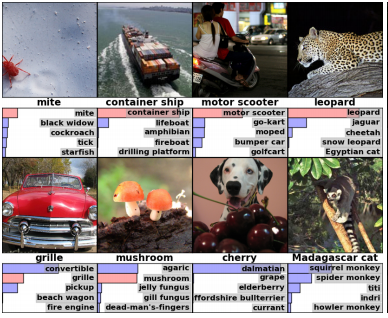
\includegraphics[width=0.95\textwidth]{result.jpg}
     \caption {Convergence Curve }
     \label{cc}
\end{center}
\end{figure}
According to the figure \ref{cc}, convergence behavior analysis shows that  GWO tend to extensively search promising regions of the search spaces and exploit the best one.
%\par TGWO can converge to the
%optimal value 0 by optimizing the unimodal functions F1-
%F4 and F18-F19; For functions F5 and F9, TGWO has the
%best optimization effect, followed by TSGWO; The average value of the optimization function F6 of the SSA algorithm is the closest to the optimal solution and the standard
%deviation is the smallest. 

\chapter{Conclusion}
Studied about grey wolf hierarchy and observed the various phases of grey wolf hunting.
Mimicked the social hierarchy and hunting behaviour of grey wolves.
Twenty nine test functions were employed to benchmark the performance of GWO in terms of exploration, exploitation, local optima  avoidance,  and  convergence.
Unimodal functions showed the superior exploitation of the GWO algorithm. 
The exploration ability of GWO  was  confirmed  by  the  results  on  multimodal  functions.  
The  composite  functions showed high local optima avoidance. 
The convergence analysis of GWO confirmed the convergence of this algorithm. 

\bibliographystyle{unsrt}
\bibliography{references.bib}
\cite{one}
\cite{two}
\cite{three}
\cite{four}
\cite{five}

%\begin{appendices}
%\addtocontents{toc}{\protect\setcounter{tocdepth}{0}}
%\chapter{Questionnaire}
%
%\end{appendices}




\end{document}